\documentclass{exam}
\usepackage[utf8]{inputenc}
\usepackage{lmodern}
\usepackage{microtype}

% \usepackage[parfill]{parskip}
\usepackage[dvipsnames]{xcolor}
\usepackage{amsmath}
\usepackage{amsfonts}
\usepackage{amsthm}
\usepackage{siunitx}
\DeclareSIUnit\year{yr}
\DeclareSIUnit\foot{ft}
\DeclareSIUnit\litre{\liter}

\usepackage{skull}

\usepackage{pgfplots}
\usepgfplotslibrary{polar}
\pgfplotsset{compat=1.11}
\usepgfplotslibrary{statistics}
\usepackage{graphicx}
\usepackage{sidecap}
\sidecaptionvpos{figure}{c}
\usepackage{float}
\usepackage{gensymb}
\usepackage{tkz-euclide}
\usetkzobj{all}
\usepackage{commath}
\usepackage{hyperref}
\usepackage{enumitem}
\usepackage{wasysym}
\usepackage{multicol}
\usepackage{mathtools}
\usepackage{tcolorbox}
\usepackage{tabularx}
\usepackage[version=4]{mhchem}
\usepackage{changepage}
\usepackage{listings}
\lstset{basicstyle=\ttfamily\linespread{0.8}\small}

\renewcommand*{\thefootnote}{\fnsymbol{footnote}}

\newtheorem*{thm}{Theorem}
\newtheorem*{iden}{Identity}
\newtheorem*{lemma}{Lemma}
\newtheorem{obs}{Observation}
\theoremstyle{definition}
\newtheorem*{defn}{Definition}
\newtheorem*{ex}{Example}
\newtheorem{con}{Construction}
\newtheorem*{alg}{Algorithm}

\newtheoremstyle{break}
  {\topsep}{\topsep}%
  {\itshape}{}%
  {\bfseries}{}%
  {\newline}{}%
\theoremstyle{break}
\newtheorem*{bthm}{Theorem}

% russian integral
\usepackage{scalerel}
\DeclareMathOperator*{\rint}{\scalerel*{\rotatebox{17}{$\!\int\!$}}{\int}}

% \DeclareMathOperator*{\rint}{\int}

\pgfplotsset{vasymptote/.style={
    before end axis/.append code={
        \draw[densely dashed] ({rel axis cs:0,0} -| {axis cs:#1,0})
        -- ({rel axis cs:0,1} -| {axis cs:#1,0});
    }
}}

% \pointsinrightmargin
\boxedpoints
\pointname{}

\newcommand{\questioA}{\question[\texttt{\textbf{\color{Cerulean} A}}]}
\newcommand{\questioM}{\question[\texttt{\textbf{\color{PineGreen} M}}]}
\newcommand{\questioE}{\question[\texttt{\textbf{\color{WildStrawberry} E}}]}
\newcommand{\questioS}{\question[\texttt{\textbf{\color{Goldenrod} S}}]}
\newcommand{\questioO}{\question[\texttt{\textbf{\color{BurntOrange} O}}]}

\newcommand{\parA}{\part[\texttt{\textbf{\color{Cerulean} A}}]}
\newcommand{\parM}{\part[\texttt{\textbf{\color{PineGreen} M}}]}
\newcommand{\parE}{\part[\texttt{\textbf{\color{WildStrawberry} E}}]}
\newcommand{\parS}{\part[\texttt{\textbf{\color{Goldenrod} S}}]}
\newcommand{\parO}{\part[\texttt{\textbf{\color{BurntOrange} O}}]}

\newcommand{\subparA}{\subpart[\texttt{\textbf{\color{Cerulean} A}}]}
\newcommand{\subparM}{\subpart[\texttt{\textbf{\color{PineGreen} M}}]}
\newcommand{\subparE}{\subpart[\texttt{\textbf{\color{WildStrawberry} E}}]}
\newcommand{\subparS}{\subpart[\texttt{\textbf{\color{Goldenrod} S}}]}
\newcommand{\subparO}{\subpart[\texttt{\textbf{\color{BurntOrange} O}}]}

\newcommand{\mainHeader}[2]{\section*{NCEA Level 2 Mathematics\\#1. #2}}
\newcommand{\mainHeaderHw}[2]{\section*{NCEA Level 2 Mathematics (Homework)\\#1. #2}}
\newcommand{\seealso}[1]{\begin{center}\emph{See also #1.}\end{center}}
\newcommand{\drills}[1]{\begin{center}\emph{Drill problems: #1.}\end{center}}
\newcommand{\basedon}[1]{\begin{center}\emph{Notes largely based on #1.}\end{center}}


\begin{document}

\mainHeaderHw{11}{Slopes and Differentiation}
\subsection*{Reading}
\begin{center}
\begin{tcolorbox}[width=0.8\textwidth,colback={white},title={\textbf{Go and watch...}},colbacktitle=black,coltitle=white]
  \textcolor{black}{\url{https://www.youtube.com/watch?v=axZTv5YJssA}}
\end{tcolorbox}
\end{center}

\begin{center}
\begin{tcolorbox}[width=0.8\textwidth,colback={white},title={\textbf{What's it good for?}},colbacktitle=MidnightBlue,coltitle=white]
  People use calculus for...
  \begin{itemize}
    \item Engineering and physics: calculus is the natural language of any system which moves or changes over time (the movement of
          a vehicle or a robot arm, or the current in an electrical system).
    \item Chemistry and biology: rates of reaction and fluid pressure, population growth, and molecular kinetics are all examples of
          systems that are best understood using either calculus or further applications of calculus.
    \item Mathematics: the subjects which grow out of calculus (analysis and topology, for example) are fundamental geometric theories
          of space, distance, and transformation.
  \end{itemize}
\end{tcolorbox}
\end{center}

\subsection*{Questions}
\begin{questions}
  \question A function $ f $ is given by $ f(x) = 2x^3 - 10x + 5 $. Find the gradient of the graph of $ f $ at the point where $ x = 2 $.
  \question Find the coordinates of the point on the curve $ y = \frac{4}{x^2} $ where the gradient is 1.
  \question Answer the following questions about this graph. Open circles denote locations
            where the function \emph{is not} defined, while filled circles denote locations at
            the end of a segment where the function \emph{is} defined.
            \begin{center}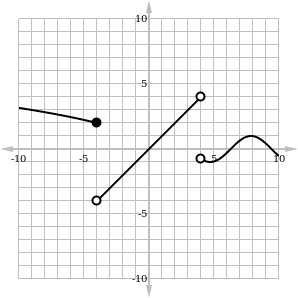
\includegraphics[width=0.3\textwidth]{fungraph}\end{center}
    \begin{parts}
      \part What is the slope of the graph at $ x = 8 $?
      \part Does the function have a derivative everywhere (i.e. can you guess the slope of the graph at every point)? If not, where
            does it fail to be differentiable?
      \part At $ x = -5 $, is the derivative positive or negative?
      \part What is the slope of the curve around $ x = 0 $?
    \end{parts}
\end{questions}

\end{document}
